\begin{ejercicio}
	Teniendo la forma de cada operador y sabiendo que $[x,p] = i\hbar$, entonces
	$$
		[a,a^\dagger] = \frac{m\omega}{2\hbar} \qty[ x + \frac{ip}{m\omega}, x - \frac{ip}{m\omega} ] = \frac{m\omega}{2\hbar} \qty(-\frac{2i}{m\omega} [x,p]) = \mathbb{1} .
	$$
\end{ejercicio}

\begin{ejercicio}
	Tomando los operadores de creación y aniquilación, se tiene
		$$
			aa^\dagger = \frac{m\omega}{2\hbar} \qty(x^2 + \frac{p^2}{m^2 \omega ^2} + \frac{i}{m\omega} [x,p]) + \frac{1}{2} \hbar \omega = \frac{1}{2} m\omega ^2 x^2 + \frac{p^2}{2m} .
		$$
\end{ejercicio}

\begin{ejercicio}
	Teniendo las definiciones de los operadores de creación y aniquilación 
	$$
		\left.\begin{array}{ccc}
			a\ket{n} & = & \sqrt{n} \ket{n - 1} \\
			a^\dagger \ket{n} & = & \sqrt{n + 1} \ket{n + 1} \\
		\end{array}\right\}
		\Rightarrow \left\{\begin{array}{ccc}
			a^2 \ket{n} & = & \sqrt{n(n - 1)} \ket{n - 2} \\
			a^{\dagger ^{2}} \ket{n} & = & \sqrt{(n + 1)(n + 2)} \ket{n + 2} 
		\end{array}\right. .
	$$
	Calulamos los operadores $X$ y $P$ en términos de $a$ y $a^\dagger$
	\begin{align*}
		X &= \sqrt{\frac{\hbar}{2m\omega}} \qty(a^\dagger + a) \\
		P &= m\omega i \sqrt{\frac{\hbar}{2m\omega}} \qty(a^\dagger - a) \\
		X^2 &= \frac{\hbar}{2m\omega} \qty(a^{\dagger ^{2}} + a^\dagger a + aa^\dagger + a^2) \\
		P^2 &= -\qty(\frac{m\omega \hbar}{2})^2 \qty(a^{\dagger ^{2}} + a^2 - a^\dagger a - aa^\dagger) .
	\end{align*}
	Encontrando
	\begin{align*}
		\mel{m}{x}{n} &= \mel{m}{\sqrt{\frac{\hbar}{2m\omega}} \qty(a^\dagger + a)}{n} \\
			&= \sqrt{\frac{\hbar}{2m\omega}} \qty(\sqrt{n + 1} \braket{m}{n + 1} + \sqrt{n} \braket{m}{n - 1}) \\
			\Aboxed{ &= \sqrt{\frac{\hbar}{2m\omega}} \qty(\sqrt{n + 1} \delta_{m,n + 1} + \sqrt{n} \delta_{m,n - 1})}
	\end{align*}
	bajo la misma idea
	\begin{align*}
		\Aboxed{ \mel{m}{p}{n} &= \sqrt{\frac{\hbar m \omega}{2}} i \qty( \sqrt{n + 1} \delta_{m,n + 1} - \sqrt{n} \delta_{m,n - 1} ) }.
	\end{align*}
	\begin{align*}
		\mel{m}{x^2}{n} &= \frac{\hbar}{2m\omega} \bra{m} \qty[\sqrt{(n + 1)(n + 2)} \ket{n + 2} + \sqrt{n(n - 1)} \ket{n - 2} + n\ket{n} + (n + 1)\ket{n}] \\
		\Aboxed{ &= \frac{\hbar}{2m\omega} \qty(\sqrt{(n + 1)(n + 2)} \delta_{m,n + 2} + \sqrt{n(n - 1)} \delta_{m,n - 2} + n\delta_{m,n} + (n + 1)\delta_{m,n}) }
	\end{align*}
	\begin{align*}
		\Aboxed{ \mel{m}{p^2}{n} &= -\frac{m\omega \hbar}{2} \qty( \sqrt{(n + 1)(n + 2)}\delta_{m,n + 2} + \sqrt{n(n - 1)} \delta_{m,n - 2} - n\delta_{m,n} - (n + 1) \delta_{m,n} ) }
	\end{align*}
	y
	\begin{align*}
		\Aboxed{ \mel{m}{[x,p]}{n} &= i\hbar \delta_{m,n} }
	\end{align*}
\end{ejercicio}

\begin{ejercicio}
	Tomando únicamente el signo $+$, se tiene
	\begin{align*}
		[J_z , J_+] &= \frac{\hbar ^2}{2} \qty[a_+ ^\dagger a_+ -a_- ^\dagger a_- ,a_+ ^\dagger a_-].
	\end{align*}
	Utilizando la propiedad $[AB,C] = A[B,C] + [A,C]B$, se tiene
	$$ [a_+ ^\dagger a_+,a_+ ^\dagger a_-] = a_+ ^\dagger \underbrace{[a_+,a_+ ^\dagger a_-]}_{a_-} + \underbrace{[a_+ ^\dagger ,a_+ ^\dagger a_]}_{0} a_+ = a_+ ^\dagger a_-$$
	$$ [a_- ^\dagger a_-,a_+ ^\dagger a_-] = a_- ^\dagger \underbrace{[a_-,a_+ ^\dagger a_-]}_{0} + \underbrace{[a_- ^\dagger ,a_+ ^\dagger a_]}_{-a_+ ^\dagger} a_- = -a_+ ^\dagger a_-,$$
	entonces
	$$ \boxed{ [J_z , J_+] = \hbar J_+ } $$
	La misma idea para $J_-$.
\end{ejercicio}

\begin{ejercicio}
	Teniendo las funciones $\varphi _{0,1} (x)$
		$$ \varphi _0 (x) = \frac{e^{-\frac{x^2}{2}}}{\sqrt[4]{\pi }} $$
		$$ \varphi _1 (x) = \frac{\sqrt{2} e^{-\frac{x^2}{2}} x}{\sqrt[4]{\pi }}, $$
	Aplicamos el hamiltoniano $H = \frac{1}{2} p^2 + \frac{1}{2} x^2$ con $p = -i\dv{x}$, lo que nos da
		$$ H \varphi _0 (x) = \frac{e^{-\frac{x^2}{2}}}{2 \sqrt[4]{\pi }} = \frac{1}{2} \varphi _0 (x), $$
	y
		$$ H \varphi _1 (x) = \frac{3 e^{-\frac{x^2}{2}} x}{\sqrt{2} \sqrt[4]{\pi }} = \frac{3}{2} \varphi _1 (x). $$
	Ahora, si definimos otra función
		$$ \varphi _2 (x) = \frac{e^{-\frac{x^2}{2}} \left(\alpha x^2-1\right)}{\sqrt{2} \sqrt[4]{\pi }}, $$
	de modo que sea ortogonal a $\varphi _0 (x)$ y $\varphi _1 (x)$, se encuentra el valor de $\alpha$. Para ello utilizamos mathematica, y el resultado de los productos internos respectivos, se tiene
		$$ \int _{-\infty} ^\infty \dd{x} \varphi _0 (x) \varphi _2 ^* (x) = \frac{\alpha -2}{2 \sqrt{2}} $$
	y
		$$ \int _{-\infty} ^\infty \dd{x} \varphi _1 (x) \varphi _2 ^* (x) = 0. $$
	Entonces el valor de $\alpha = 2$. Aplicando el hamiltoniano, vemos que también es función propia de él, con valor propio $\flatfrac{5}{2}$
		$$ H \varphi _2 (x) = \frac{5 e^{-\frac{x^2}{2}} \left(2 x^2-1\right)}{2 \sqrt{2} \sqrt[4]{\pi }} = \frac{5}{2} \varphi _2 (x). $$
\end{ejercicio}

\begin{ejercicio}
	Tomando el operador creación
		$$ a^\dagger = \sqrt{\frac{m\omega}{2\hbar}} \qty(x - \frac{\hbar}{m\omega}  \dv{x}); $$
	además, sabiendo que $\braket{x}{2} = \frac{1}{\sqrt{2}} \mel{x}{a^{\dagger ^{2}}}{0}$ y que
		$$ \braket{x}{0} = \varphi _o (x) = \qty(\frac{m\omega}{2\hbar})^{\flatfrac{1}{4}} e^{-\frac{m\omega}{2\hbar} x^2}. $$
	Entonces, sustituyendo las relaciones obtenidas ateriormente se llega a $\varphi _2 (x)$, 
		$$ \varphi _2 (x) = \frac{1}{\sqrt{2}} \qty(\frac{m\omega}{\pi \hbar})^{\flatfrac{1}{4}} \qty(\frac{2m\omega}{\hbar} x^2 - 1) e^{-\frac{m\omega}{2\hbar} x^2} $$
	\begin{figure}[H]
		\centering
		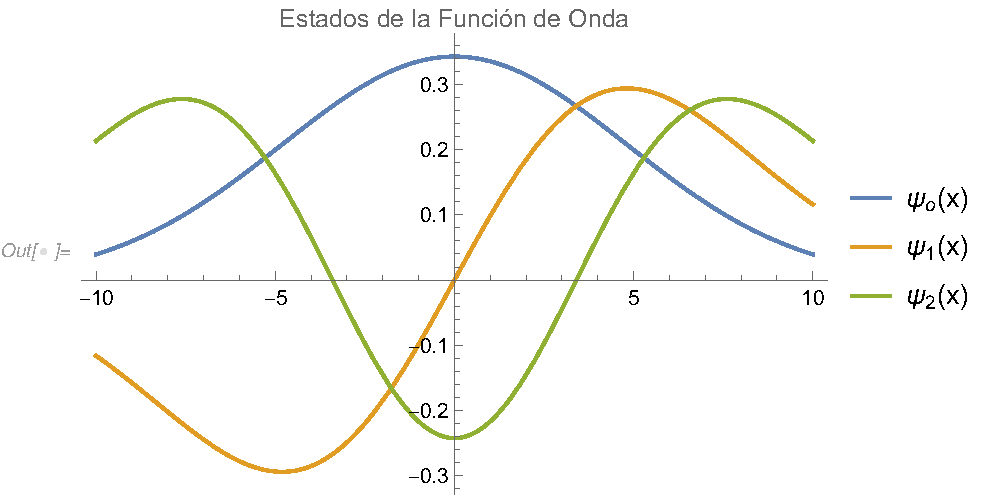
\includegraphics[scale=0.75]{img/graphs.pdf}
		\caption{Gráfica de las funciones de onda $\varphi _{0,1,2} (x)$.}
		\label{graphs}
	\end{figure}
	Para el útlimo inciso, ver el script de mathematica.
\end{ejercicio}












%%%%%%%5